% Created 2016-08-17 Wed 14:38
\documentclass[tikz]{standalone}

\usepackage[utf8]{inputenc}
\usepackage[T1]{fontenc}
\usepackage{helvet}
\usepackage{../../templates/msc}

\renewcommand{\familydefault}{\sfdefault}

\tikzset{
every picture/.style={
line width=1pt
}}

\usepackage{tikz}
\author{Holger Karl}
\date{\today}
\title{}


\usetikzlibrary{shapes}

\begin{document}
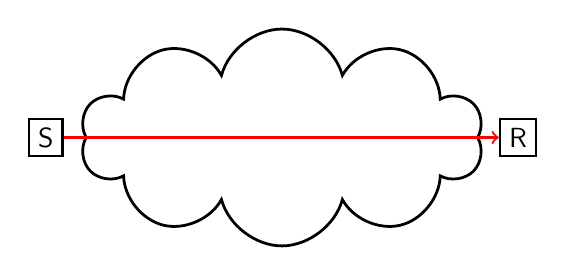
\begin{tikzpicture}[auto,
block/.style = {rectangle, draw=black, thick, align=left}]

\node[block] (s) at (0,0) {S}; 
\node[block] (r) at (6,0) {R}; 
\node[draw, cloud, aspect=3, scale=5] (c) at (3,0) {};
\draw [red, thick, ->] (s) -- (r);
\end{tikzpicture}

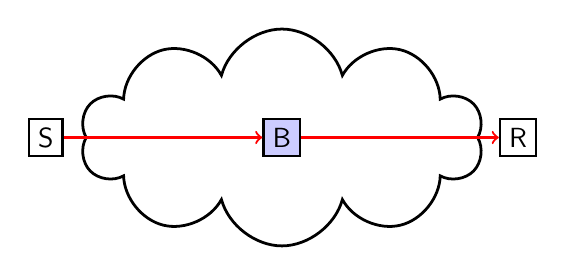
\begin{tikzpicture}[auto,
block/.style = {rectangle, draw=black, thick, align=left}]

\node[block] (s) at (0,0) {S}; 
\node[block] (r) at (6,0) {R}; 
\node[draw, cloud, aspect=3, scale=5] (c) at (3,0) {};

\node[draw, rectangle,thick, fill=blue!20] (b) at (3,0) {B};

\draw [red, thick, ->] (s) -- (b); 
\draw [red, thick, ->] (b) -- (r); 
\end{tikzpicture}

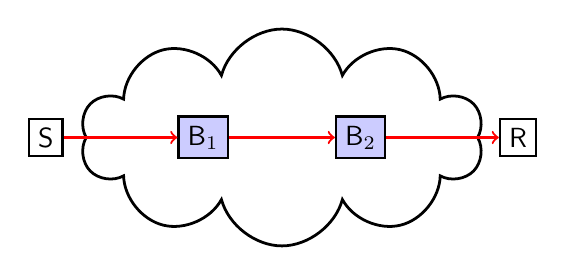
\begin{tikzpicture}[auto,
block/.style = {rectangle, draw=black, thick, align=left}]

\node[block] (s) at (0,0) {S}; 
\node[block] (r) at (6,0) {R}; 
\node[draw, cloud, aspect=3, scale=5] (c) at (3,0) {};

\node[draw, rectangle,thick, fill=blue!20] (b1) at (2,0) {B$_1$}; 
\node[draw, rectangle,thick, fill=blue!20] (b2) at (4,0) {B$_2$}; 

\draw [red, thick, ->] (s) -- (b1); 
\draw [red, thick, ->] (b1) -- (b2); 
\draw [red, thick, ->] (b2) -- (r); 
\end{tikzpicture}

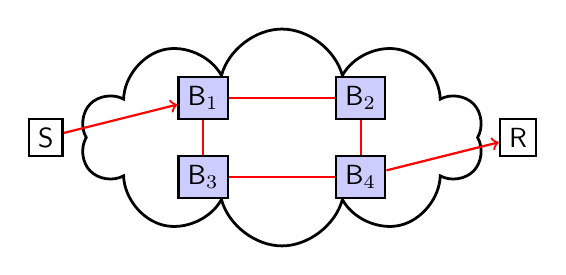
\begin{tikzpicture}[auto,
block/.style = {rectangle, draw=black, thick, align=left}]

\node[block] (s) at (0,0) {S}; 
\node[block] (r) at (6,0) {R}; 
\node[draw, cloud, aspect=3, scale=5] (c) at (3,0) {};

\node[draw, rectangle,thick, fill=blue!20] (b1) at (2,0.5) {B$_1$}; 
\node[draw, rectangle,thick, fill=blue!20] (b2) at (4,0.5) {B$_2$}; 
\node[draw, rectangle,thick, fill=blue!20] (b3) at (2,-0.5) {B$_3$}; 
\node[draw, rectangle,thick, fill=blue!20] (b4) at (4,-0.5) {B$_4$}; 

\draw [red, thick, ->] (s) -- (b1); 
\draw [red, thick] (b1) -- (b2); 
\draw [red, thick] (b1) -- (b3); 
\draw [red, thick] (b2) -- (b4); 
\draw [red, thick] (b3) -- (b4); 
\draw [red, thick, ->] (b4) -- (r); 
\end{tikzpicture}


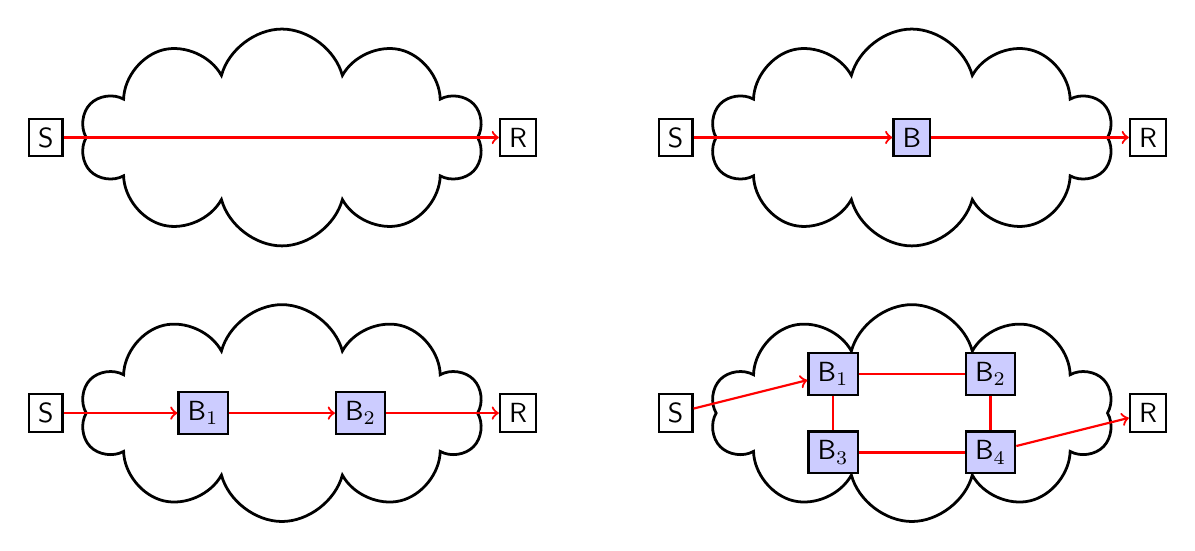
\begin{tikzpicture}[auto,
block/.style = {rectangle, draw=black, thick, align=left}]
\begin{scope}
\node[block] (s) at (0,0) {S}; 
\node[block] (r) at (6,0) {R}; 
\node[draw, cloud, aspect=3, scale=5] (c) at (3,0) {};
\draw [red, thick, ->] (s) -- (r);
\end{scope}

\begin{scope}[xshift=8cm]
\node[block] (s) at (0,0) {S}; 
\node[block] (r) at (6,0) {R}; 
\node[draw, cloud, aspect=3, scale=5] (c) at (3,0) {};

\node[draw, rectangle,thick, fill=blue!20] (b) at (3,0) {B};

\draw [red, thick, ->] (s) -- (b); 
\draw [red, thick, ->] (b) -- (r);   
\end{scope}


\begin{scope}[yshift=-3.5cm]
\node[block] (s) at (0,0) {S}; 
\node[block] (r) at (6,0) {R}; 
\node[draw, cloud, aspect=3, scale=5] (c) at (3,0) {};

\node[draw, rectangle,thick, fill=blue!20] (b1) at (2,0) {B$_1$}; 
\node[draw, rectangle,thick, fill=blue!20] (b2) at (4,0) {B$_2$}; 

\draw [red, thick, ->] (s) -- (b1); 
\draw [red, thick, ->] (b1) -- (b2); 
\draw [red, thick, ->] (b2) -- (r);   
\end{scope}

\begin{scope}[xshift=8cm, yshift=-3.5cm]
  \node[block] (s) at (0,0) {S}; \node[block] (r) at (6,0) {R};
  \node[draw, cloud, aspect=3, scale=5] (c) at (3,0) {};

  \node[draw, rectangle,thick, fill=blue!20] (b1) at (2,0.5) {B$_1$};
  \node[draw, rectangle,thick, fill=blue!20] (b2) at (4,0.5) {B$_2$};
  \node[draw, rectangle,thick, fill=blue!20] (b3) at (2,-0.5) {B$_3$};
  \node[draw, rectangle,thick, fill=blue!20] (b4) at (4,-0.5) {B$_4$};

  \draw [red, thick, ->] (s) -- (b1); \draw [red, thick] (b1) -- (b2);
  \draw [red, thick] (b1) -- (b3); \draw [red, thick] (b2) -- (b4);
  \draw [red, thick] (b3) -- (b4); \draw [red, thick, ->] (b4) -- (r);
\end{scope}
\end{tikzpicture}


\end{document}